\section{Holiday and Sick Leave Detection}

The information about anomalies in the regular work pattern can be a valuable information for several parties.
Usually only few parties know about the holiday or sick leave times of a person.
To know if a persons tends to become sick more often or for long times is a dangerous intrusion into a persons privacy.
For instance this could be abused by head hunters or personnel managers to cull possible employees with too high sick leave rates and thereby reduce the job prospects of the target.

For employers this might be convenient for detecting anomalies in the productivity of employees.
In case an employee does not commit on a regular basis for several days, this behaviour would be instantly visible with this method.

Another attack vector could be to look at the correlation of miss-out between several persons.
This attack could even be performed by an outsider on a commercial open-source project, if the employees of the targeted company are known.
The information gained by this attack could be quite delicate, as it could reveal relationships between persons.
This attack is heavily inspired by an article about data mining articles from the popular German weekly magazine \emph{Der Spiegel} written by the David Kriesel~\cite{article:spiegel-mining}.

For now the goal of this attack is to simply detect miss-out and if a contributor has anomalies in their regular work day pattern.


\subsection{Implementation}

Due to possible fluctuations or changes in work routine, one requirement to this algorithm is the detection of a regular work pattern for a given interval.
It must have the ability to adjust to a changing work pattern, but at the same time it needs to be capable of detecting anomalies in this pattern.

The input for this analysis is the intersection between all commits from the considered repositories and all commits from the considered contributors.
The commits' meta data used for this analysis are timestamps as well as additions and deletions in lines of code.

\begin{figure}[H]
    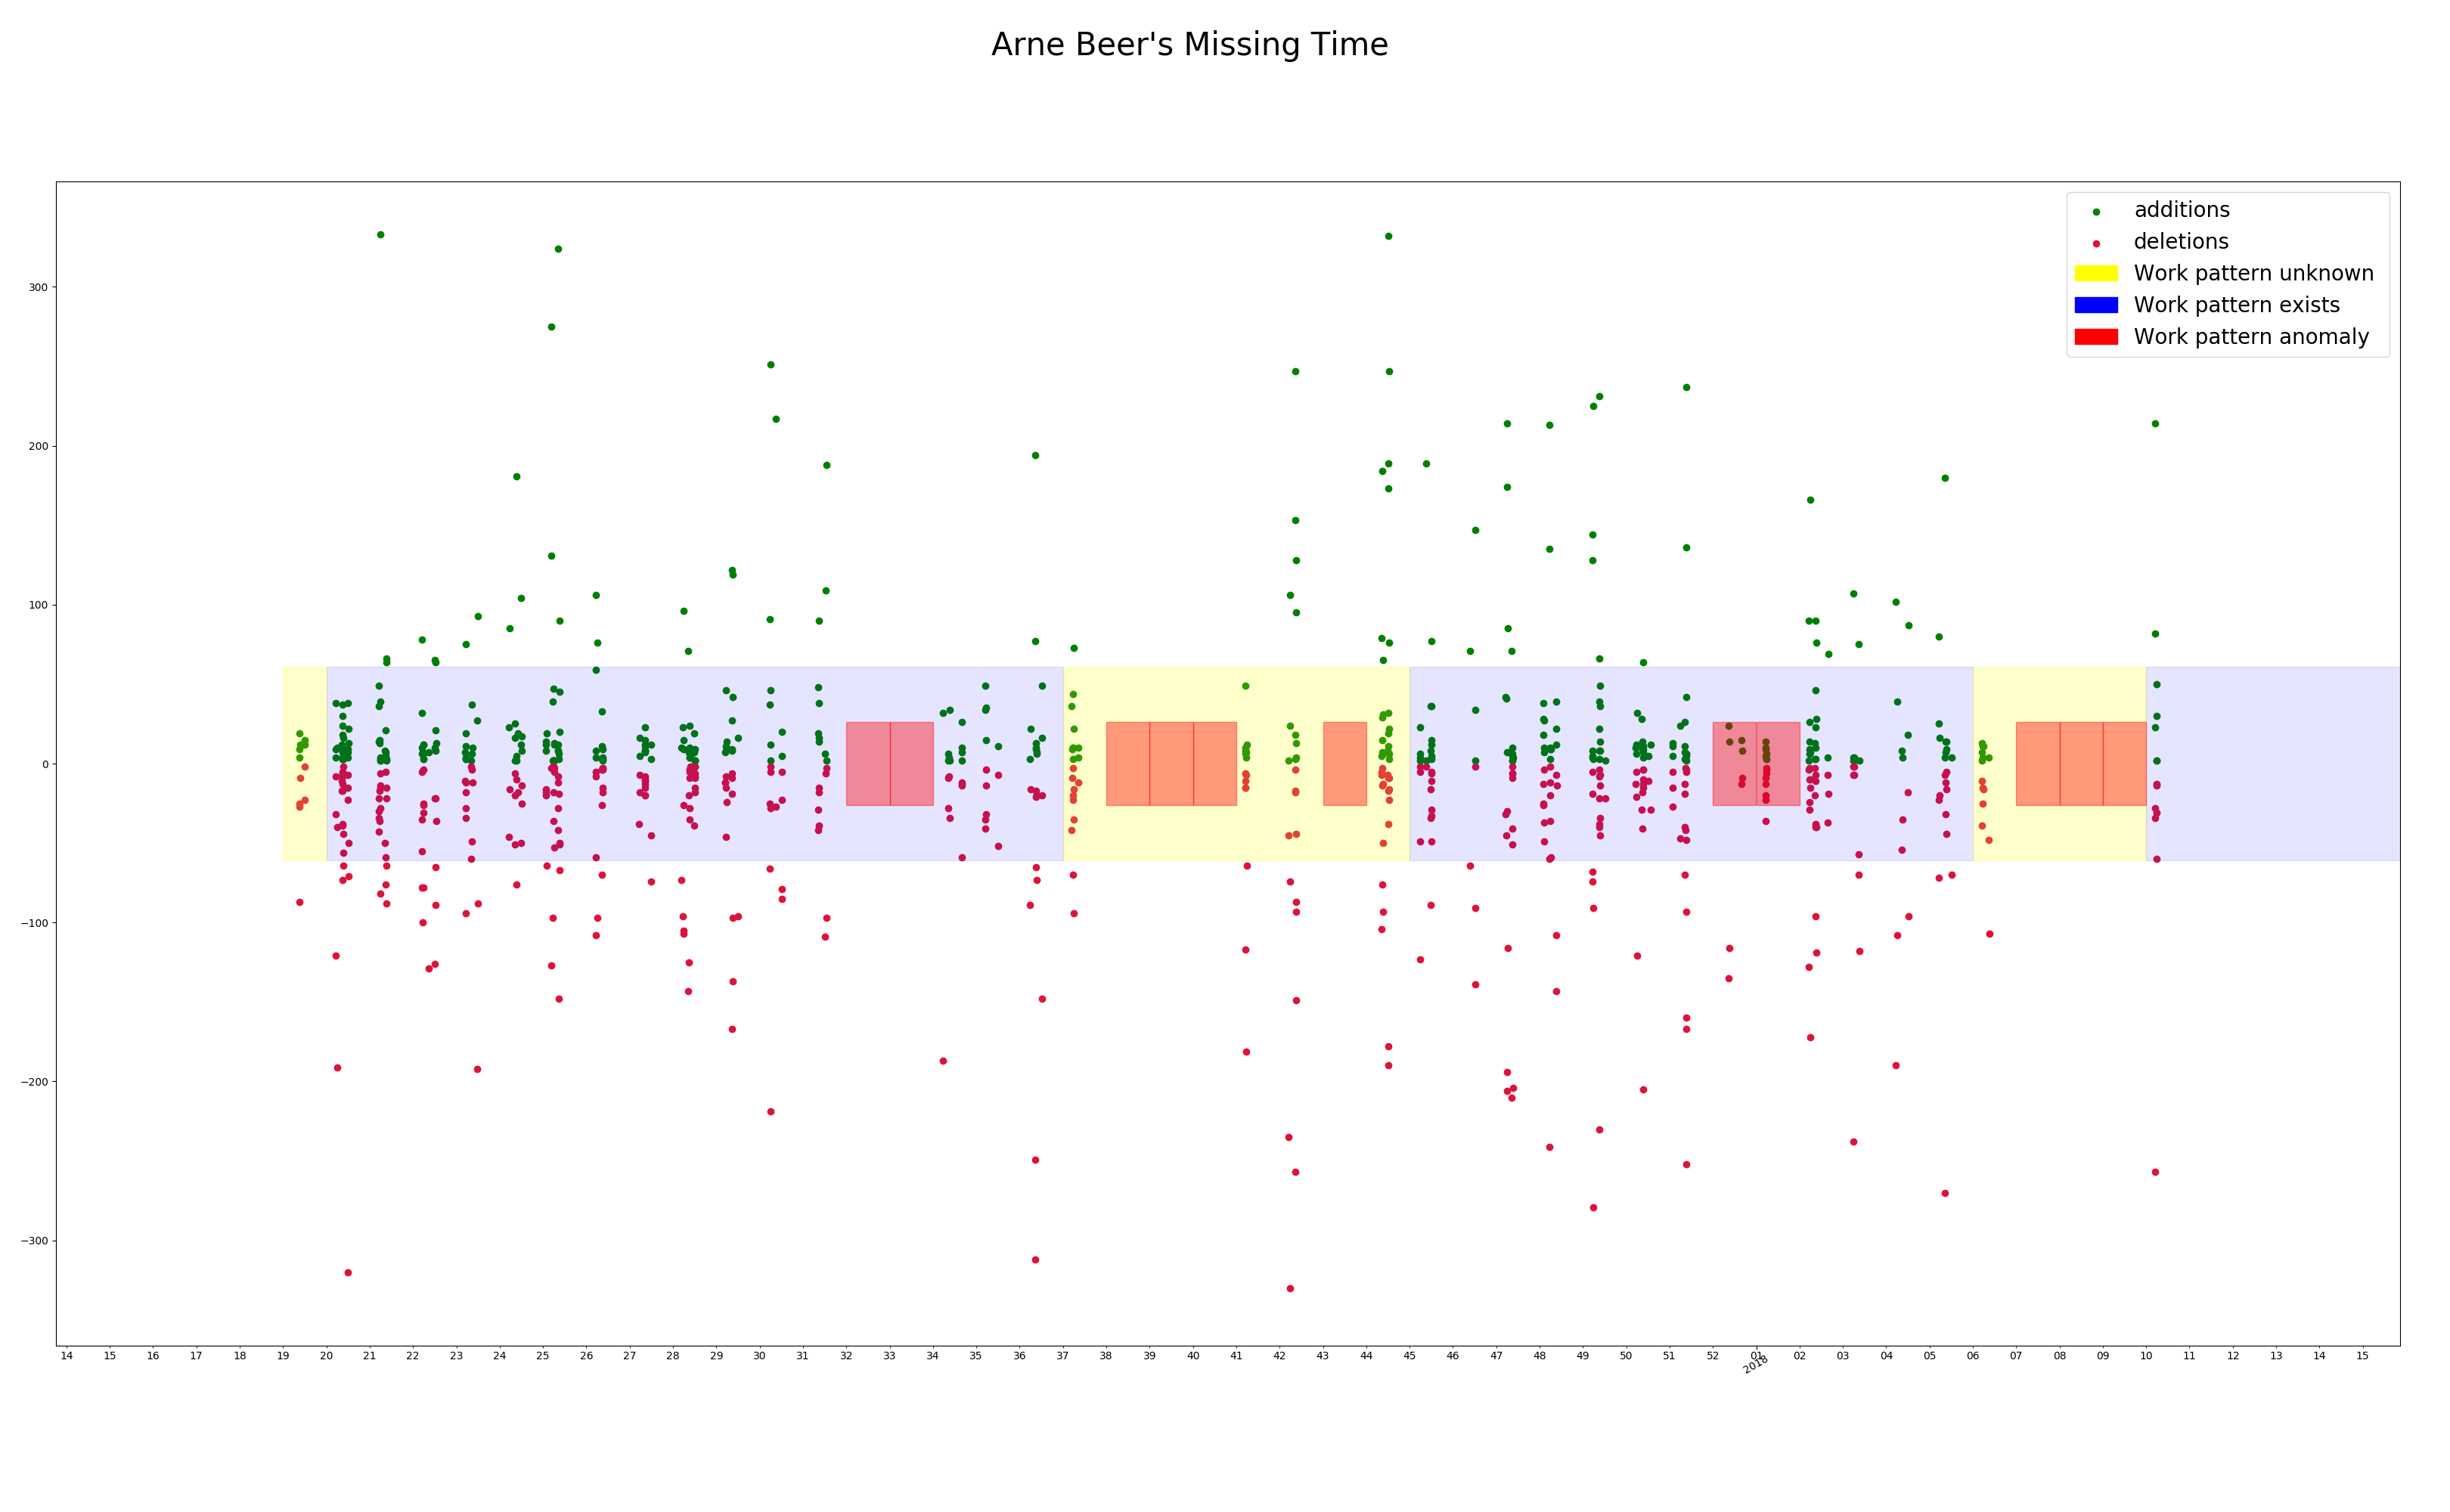
\includegraphics[scale=0.20]{./graphs/analysis/work-time-analysis}
    \centering
    \caption{The work time analysis of the author.}\label{fig:missing-time}
\end{figure}

The analysis of the data is a chronological scan of all commits for specific user.
Before performing the actual analysis, the data is converted into an easier to handle format.
It is really difficult to measure productivity in lines of code or in the amount of commits made by a person, as they do not necessarily display the amount of work, which has been put into this code.
As a result I decided, that a day counts as a work day as long as at least a single commit is created during the day.
The preprocessed data is thereby equivalent to the days a contributor worked on, ordered by the week of the year.

\begin{minted}[linenos]{python}
def analyse(weeks):
    prototype = None
    for index, week in weeks.items():
        next_six_weeks = weeks[index:index+future_lookup]
        if not prototype:
            # See if there is a prototype in the next few weeks.
            prototype = find_prototype(next_six_weeks)

            # Check if this specific week is a anomaly
            check_anomaly(prototype, week)

            continue

        prototype_exists = prototype_exists_in_next_weeks(next_six_weeks)
        if not prototype_exists:
            # We couldn't find the prototype in the next few rows
            # Try to find a new prototype
            prototype = find_prototype(next_six_weeks)

        check_anomaly(prototype, week)


def check_anomaly(prototype, week):
    if week.working_days == 0:
        save_anomaly(week)

    if prototype is not None:
        different_days = week.working_days - prototype.working_days
        // A single day variance is acceptable
        if different_days >= 1:
            save_anomaly(week)

\end{minted}
\begingroup
\captionof{listing}{Miss-out analysis algorithm.}\label{lst:miss-out-algorithm}
\endgroup

The algorithm inspects every week work pattern of a given interval, which has been set to a year for this analysis.
At the beginning, a new \emph{prototype} is tried to be found.
This is performed in the function \inlinecode{find\_prototype} in Listing\ref{lst:miss-out-algorithm}.
A prototype is a representative week work pattern, which resembles the average work day pattern of the next weeks.

This function performs a simple iteration over a fix amount of future weeks, to find a work day pattern occurring more often than a given threshold.
If a prototype is found, we are capable of identifying anomalies that deviate from this pattern.

For each following week it is then firstly checked if this week is a anomaly in regards to the current prototype.
Anomalies are simply detected by comparing the amount of working days of the prototype and the considered week.
The difference in the working patterns is not suitable for this analysis, as it produces too many false positives for employees with flexible work time.

Secondly it is checked if a week identical to the prototype exists in the near future.
If there is no such week, the current prototype is reset and a new prototype needs to be found again.

In case no prototype can be found, anomalies cannot be easily identified, as there exists no pattern to check against.
Only obvious anomalies, namely weeks without a single work day, will then be marked as such.
